\section{Approach}
\label{sec:model}
In this section we describe our approach in detail.
\figref{fig:model} gives an overview of the proposed architectures.
First we introduce the most common and popular BiLSTM-CRF
model (\figref{fig:model}(a)) for sequence labeling tasks.
Then we move on to multi-task learning perspective 
(\figref{fig:model}(b) and (c)).
Finally we propose our new method, which is called
Deep Cascade Multi-task Learning in \figref{fig:model}(d).

\begin{figure}[th]
	\centering
	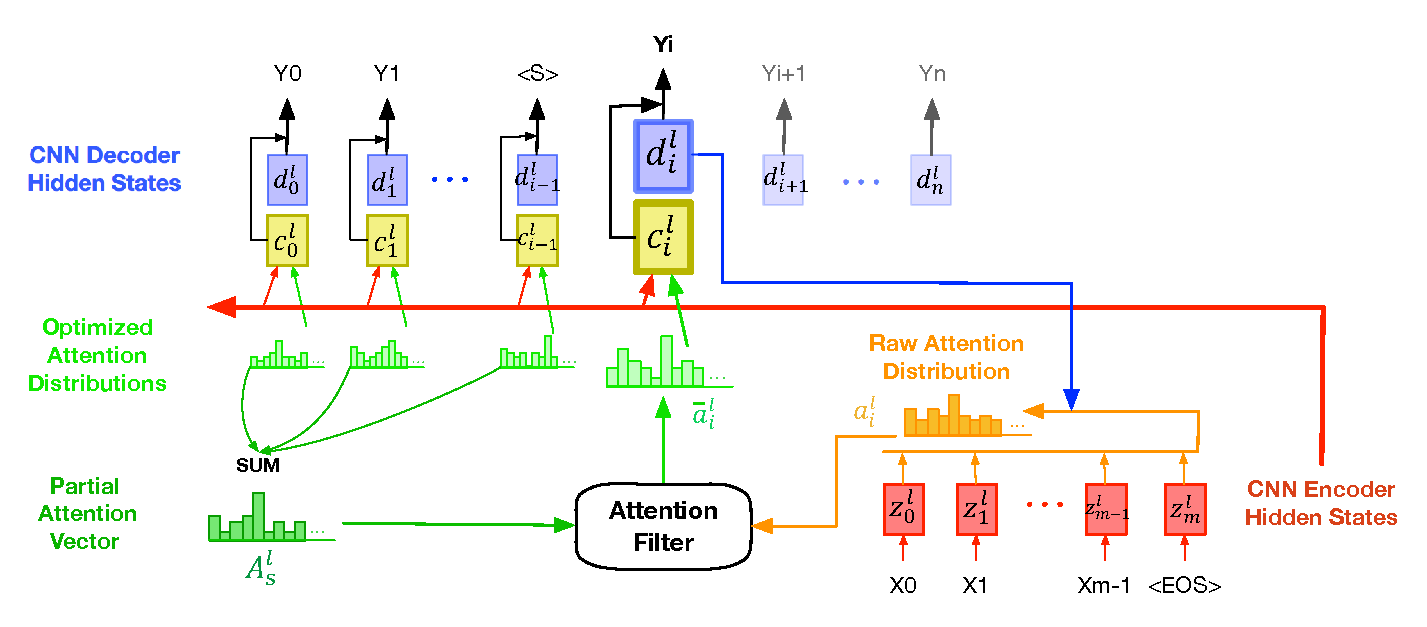
\epsfig{file=figures/model.eps, width=1.0\columnwidth}
	\caption{Sequential models for slot filling task.}
	\label{fig:model}
	\vspace{-10pt}
\end{figure}

\subsection{RNN Sequence Labeling}
\label{sec:rnn_sequence_labeling}

\figref{fig:model}(a) 
shows the principle architecture of a BiLSTM-CRF model,
which is the state-of-the-art model for various sequence labeling tasks \cite{huang2015bidirectional,reimers2017optimal}.
BiLSTM-CRF model consists of a BiLSTM layer and a CRF layer. 

Bidirectional LSTMs enable the
hidden states to capture both historical and future
context information of the words.
Mathematically, the input of this BiLSTM layer
is a sequence of input vectors,
denoted as $\bi{X}=(\bi{x}_1, \bi{x}_2, ..., \bi{x}_T)$.
The output of BiLSTM layer is a sequence of the hidden
states for each input word, denoted
as $\bi{H}=(\bi{h}_1, \bi{h}_2, ..., \bi{h}_T)$.
Each final hidden state is the concatenation of the forward
$\overrightarrow{\bi{h}_i}$ and backward $\overleftarrow{\bi{h}_i}$ hidden states.
We view BiLSTM as a function $\bilstm(\bi{x}_i)$:
\begin{eqnarray*}
	& \overrightarrow{\bi{h}_i} = \lstm(\bi{x}_i, \overrightarrow{\bi{h}_{i-1}}),
	\overleftarrow{\bi{h}_i} = \lstm(\bi{x}_i, \overleftarrow{\bi{h}_{i+1}}), \\
	& \bilstm(\bi{x}_i) = \bi{h}_i = [\overrightarrow{\bi{h}_i}(\bi{x}_i);\overleftarrow{\bi{h}_i}(\bi{x}_i)].
\end{eqnarray*}
Most of time we stack multiple BiLSTMs to make the model deeper,
%in which higher layer takes the output state $\bi{h}_i$ of the connected lower layer as input.
in which the output $\bi{h}_i^l$ of layer $l$ becomes the input of layer $l+1$,
e.g. $\bi{h}_i^{l+1}=\bilstm^{l+1}(\bi{h}_i^l)$.

It is always beneficial to consider the correlations
between the current label and neighboring
labels, since there are many syntactical constraints
in natural language sentences.
%For example,
%\KZ{\textbf{I-Brand} is never followed by a \textbf{B-Color}}. 
If we simply feed the above mentioned hidden states
independently to a softmax layer to predict the labels \cite{hakanni-tur2016multidomain},
such constraints are more likely
to be violated. Linear-chain Conditional Random
Field (CRF) \cite{lafferty2001conditional} 
is the most popular way to control the structure
prediction and its basic idea is to use a series
of potential functions to approximate the conditional
probability of the output label sequence
given the input word sequence.

Formally, we take the above sequence of hidden
states $\bi{H} = (\bi{h}_1, \bi{h}_2, ..., \bi{h}_T)$
as input to a CRF layer,
and the output of the CRF is the final prediction label sequence
$\bi{y} = (y_1, y_2, ..., y_T)$,
where $y_i$ is in the set of pre-defined target labels.
We denote $\mathcal{Y}(\bi{H})$ as the set of all possible label sequences.
Then we derive the conditional probability of the output sequence,
given the input hidden state sequence is:
$$
p(\bi{y}|\bi{H};\bi{W}, \bi{b})=\frac{\prod_{i=1}^{T}\varphi(y_{i-1},y_i,\bi{H})}
{\sum_{\bi{y}'\in\mathcal{Y}(\bi{H})}\prod_{i=1}^{T}\varphi(y'_{i-1},y'_i,\bi{H})},
$$
where $\varphi(y',y,\bi{H})=\exp(\bi{W}_{y',y}^{T}\bi{H}+\bi{b}_{y',y})$ are potential functions and $\bi{W}_{y',y}^{T}$ and $\bi{b}_{y',y}$ are weight vector and bias of label pair $(y', y)$.
To train the CRF layer, we use the classic maximum
conditional likelihood estimate and gradient ascent.
For a training dataset $\{(\bi{H}_{(i)}, \bi{y}_{(i)})\}$, 
the final log-likelihood is:
$$
L(\bi{W},\bi{b}) = \sum_{i}\log p(\bi{y}_{(i)}|\bi{H}_{(i)};\bi{W},\bi{b}).
$$
Finally, the Viterbi algorithm is adopted
to decode the optimal output sequence $\bi{y}^{*}$:
$$
\bi{y}^{*}=\mathop{\arg\max}_{\bi{y}\in\mathcal{Y}(\bi{H})}p(\bi{y}|\bi{H};\bi{W},\bi{b}).
$$

\subsection{Multi-task Learning}
% Why Multi-task Learning and what's multi-task in our problem?
%\yu{Tell a story why multi-task.}
%The slot labels are informative and diverse in the case of 
%E-commerce,
%and the syntactic structure of input Chinese utterance 
%are complicated,
%so that the slot filling problem becomes hard to solve.
%If we directly train an end-to-end sequential model,
%the tagging performance will suffer from data sparsity severely.
%%Slot filling (can be seen as semantic labeling task),
%%some low-level tasks such as named entity tagging or segment tagging %(can be seen as syntactic labeling task)
%%may first make mistakes for the sparsity problem.
%%If the low-level tasks get wrong, so as to the target slot filling task.
%It is easy to make wrong decisions in the low-level tasks
%such as named entity tagging or segment tagging,
%if we try to fill in all the labels at once.
%Then the error will propagate and lead to a bad performance of 
%slot filling, which is our high-level target.

While directly attacking the slot filling task is hard,
low-level tasks with fewer labels are much easier to solve.
Once we know the syntactic structure of a sentence,
filling in semantic labels will become easier accordingly.
Thus, it is reasonable to solve the problem in a multi-task learning 
framework.
%since low-level tasks may help the learning of target task.
In our problem, we can devise three individual tasks: slot filling, named entity tagging and segment tagging.
Slot filling is our target task;
named entity tagging is to classify which named entity type (\textbf{PV}/\textbf{PK}/\textbf{CG}) a word is;
and segment tagging is to judge 
whether a word is begin (\textbf{B}), in (\textbf{I}) or out (\textbf{O}) of a trunking.

%Why MTL works?
In a multi-task learning (MTL) setting, 
we have several prediction tasks over the same input sequence,
where each task has its own output vocabulary (a set of task 
specified labels).
Intuitively, the three tasks do share a lot of information.
Consider the example in \tabref{tab:slot-filling-demo} again. 
Knowing the named entity type of ``黑色''(\emph{black}) being 
\textbf{B-PV}
can definitely help determine its slot label, 
which is \textbf{B-Color}.
Similarly, knowing its segment type (\textbf{B}) 
also helps with both named entity tagging and slot filling.
Thus it is reasonable for these tasks to share parameters
and learn in the same framework cooperatively.

\subsubsection{Vanilla Multi-task Learning}
The general idea of multi-task learning
is to share parameters of encoding part of the network.
As \figref{fig:model}(b) shows,
this is naturally achieved by sharing 
the $k$-layers BiLSTM part of the network across three tasks.
Based on that,
we use a separate CRF decoder for each task $t$:
$p(\bi{y}^t|\bi{H}^k;\bi{W}_t, \bi{b}_t)$,
where $\bi{W}_t$ and $\bi{b}_t$ are task-specific parameters.
This encourages the deep BiLSTM network 
to learn a hidden representation $\bi{H}^k$
which benefits all three different tasks.

\subsubsection{Hierarchy Multi-task Learning}
Previous discussion indicates that 
there is a natural order among the different tasks:
slot filling may benefit more from named entity tagging, than the other way around.
%This suggests having task supervision for low-level tasks at the lower BiLSTM layers.
%This also enables task-specific deep learning of the high-level tasks.
This motivates us to employ low-level tasks at lower BiLSTM layers,
while high level tasks are trained at higher layers.
This idea was first proposed by Anders and Yoav \cite{sogaard2016deep}.
As shown in \figref{fig:model}(c), 
instead of decoding all tasks separately at the outermost BiLSTM layer, 
we associate each BiLSTM layer
$l(t)$ with one task $t$.
Then the conditional probabilities of the output sequence for each task are:
%let the task specific classifier feed from that layer,
%e.g. $ne\_tag(\bi{x})=p_{ne}(\bi{y}^{ne}|\bi{h}^{l(ne)};\bi{W}_{ne})$ for named entity tagging task
%in layer $l(ne)$ with $\bi{y}_{ne}$ output.
%This enables deep task-specific learning for high-level tasks. 
%This means there will be layers shared by all tasks and layers that are specific to some tasks:
%\begin{eqnarray*}
%	& seg\_tag(\bi{w})=p_{seg}(\bi{y}^{seg}|\bi{h}^{l(seg)};\bi{W}_{seg}), \\
%	& \bi{h}^{l(seg)}=BiLSTM^{l(seg)}(E(\bi{w})). \\
%	& ne\_tag(\bi{w})=p_{ne}(\bi{y}^{ne}|\bi{h}^{l(ne)};\bi{W}_{ne}), \\
%	& \bi{h}^{l(ne)}=BiLSTM^{l(ne)}(\bi{h}^{l(seg)}).\\
%	& slot\_tag(\bi{w})=p_{slot}(\bi{y}^{slot}|\bi{h}^{l(slot)};\bi{W}_{slot}), \\
%	& \bi{h}^{l(slot)}=BiLSTM^{l(slot)}(\bi{h}^{l(ne)}).
%\end{eqnarray*}
\begin{eqnarray*}
	& \seg(\bi{w})=p(\bi{y}^{seg}|\bi{H}^{l(seg)};\bi{W}_{seg},\bi{b}_{seg}), \\
	& \bi{H}^{l(seg)}=\bilstm^{l(seg)}(E(\bi{w})). \\
	& \ner(\bi{w})=p(\bi{y}^{ne}|\bi{H}^{l(ne)};\bi{W}_{ne},\bi{b}_{ne}), \\
	& \bi{H}^{l(ne)}=\bilstm^{l(ne)}(\bi{H}^{l(seg)}).\\
	& \slot(\bi{w})=p(\bi{y}^{slot}|\bi{H}^{l(slot)};\bi{W}_{slot},\bi{b}_{slot}), \\
	& \bi{H}^{l(slot)}=\bilstm^{l(slot)}(\bi{H}^{l(ne)}).
\end{eqnarray*}
Here $\seg$, $\ner$ and $\slot$ represent the tasks of
segment tagging, named entity tagging and slot filling, respectively.
$E(\bi{w})$ is the word embeddings of input sequence $\bi{w}$ and 
$l(seg) < l(ne) < l(slot)$.
%$\bi{W}_t$ and $\bi{b}_t$ are task specific parameters.
We call this model hierarchy multi-task learning,
since some layers are shared by all tasks 
while the others are only related to specific tasks.

\subsection{Deep Cascade Multi-task Learning}
\label{sec:dcmtl}
Hierarchy multi-task learning share parameters among different tasks,
and allow low-level tasks help adjust the result of high-level target task.
It is effective for those tasks which are weakly correlated,
such as POS tagging, syntactic chunking and CCG supertagging \cite{sogaard2016deep}.
However, when it comes to problems where different tasks maintain a 
strict order, in another word, the performance of high-level task 
dramatically depends on low-level tasks,
the hierarchy structure is not compact and effective enough.
Therefore, we propose \emph{cascade} and \emph{residual} connections
to enable high-level tasks taking the tagging results and hidden states 
of low-level tasks as additional input. 
These connections serves as ``shortcuts'' that 
create a more closely coupled and efficient model.
We call it deep cascade multi-task learning, 
and the framework is shown in \figref{fig:model}(d).

\subsubsection{Cascade Connection}
%Similar to hierarchy multi-task model,
%we assign different tasks at different BiLSTM layers.
Here we feed the tagging output of the task at lower layer 
e.g. $\seg^*(\bi{w})$ or $\ner^*(\bi{w})$
to the upper BiLSTM layer as its additional input.
Now the hidden states of each task layer become:
\begin{eqnarray*}
	%& \seg(\bi{w})=p(\bi{y}_{seg}|\bi{H}^{l(seg)};\bi{W}_{seg}), \\
	& \bi{H}^{l(seg)}=\bilstm^{l(seg)}(E(\bi{w})), \\
	%& \ner(\bi{w})=p(\bi{y}_{ne}|\bi{H}^{l(ne)};\bi{W}_{ne}), \\
	& \bi{H}^{l(ne)}=\bilstm^{l(ne)}(\bi{W}_{Cas.}\cdot \seg^*(\bi{w})+\bi{H}^{l(seg)}), \\
	%& \slot(\bi{w})=p(\bi{y}_{slot}|\bi{H}^{l(slot)};\bi{W}_{slot}), \\
	& \bi{H}^{l(slot)}=\bilstm^{l(slot)}(\bi{W}_{Cas.}\cdot 
	\ner^*(\bi{w})+\bi{H}^{l(ne)}),
\end{eqnarray*}
where $\bi{W}_{Cas.}$ is the weight parameter for cascade connection.

At training time, $\seg^*(\bi{w})$ and $\ner^*(\bi{w})$ can be the 
true tagging outputs.
At inference time, we simply take the greedy path of our cascade model 
without doing search, where the model emits the
best $\seg^*(\bi{w})$ and $\ner^*(\bi{w})$ by Viterbi inference algorithm.
Alternatively, one can do beam search \cite{sutskever2014sequence,vinyals2015show} by maintaining a set of $k$ best partial hypotheses at each cascade layer.
However, unlike traditional seq2seq models e.g., in machine translation,
where each inference step is just based on probability of a discrete variable 
(by softmax function), our inference for tagging output is a 
structured probability distribution defined by the CRF output.
Efficient beam search method for this structured cascade model is 
left to our future work.

\subsubsection{Residual Connection}
To encourage the information sharing among different tasks,
we also introduce the residual connection,
where we add the input of a previous layer to the current input:
\begin{eqnarray*}
	%& \seg(\bi{w})=p(\bi{y}_{seg}|\bi{H}^{l(seg)};\bi{W}_{seg}), \\
	& \bi{H}^{l(seg)}=\bilstm^{l(seg)}(\bi{x}^{seg}), \\
	& \bi{x}^{l(seg)}=E(\bi{w}). \\
	%& \ner(\bi{w})=p(\bi{y}_{ne}|\bi{H}^{l(ne)};\bi{W}_{ne}), \\
	& \bi{H}^{l(ne)}=\bilstm^{l(ne)}(\bi{W}_{Cas.}\cdot \seg^*(\bi{w})+\bi{x}^{l(ne)}), \\
	& \bi{x}^{l(ne)}= \bi{H}^{l(seg)}+\bi{x}^{l(seg)}. \\
	%& \slot(\bi{w})=p(\bi{y}_{slot}|\bi{H}^{l(slot)};\bi{W}_{slot}), \\
	& \bi{H}^{l(slot)}=\bilstm^{l(slot)}(\bi{W}_{Cas.}\cdot 
	\ner^*(\bi{w})+\bi{x}^{l(slot)}), \\
	& \bi{x}^{l(slot)}= \bi{H}^{l(ne)}+\bi{x}^{l(ne)}.
\end{eqnarray*}

Deep residual learning \cite{he2016deep} is first introduced to ease the gradient vanish problem for training very deep neural networks.
Here we propose that residual connection between different layers can help for multi-task learning.

\subsubsection{Training}
\label{sec:training}
For our multi-task setting, 
we define three loss functions (refer to \secref{sec:rnn_sequence_labeling}):
$L_{seg}$, $L_{ne}$ and $L_{slot}$ for tasks of segment tagging, named entity tagging and slot filling respectively.
We construct three training set,
$D_{seg}$, $D_{ne}$ and $D_{slot}$,
where each of them (called $D_t$ generically) contains a set of 
input-output sequence pair $(\bi{w}, \bi{y}^t)$.
The input utterance $\bi{w}$ is shared across tasks, but the output $\bi{y}^t$ is task dependent.

For vanilla multi-task learning,
we define a loss function $L=\alpha L_{seg}+\beta L_{ner}+(1-\alpha-\beta)L_{slot}$, 
where $\alpha$ and $\beta$ are hyper-parameters.
%And we update the model parameters by loss $L$.

As for hierarchy multi-task learning and cascade multi-task learning,
we choose a random task $t$ at each training step,
followed by a random training batch $\batch(\bi{w}, \bi{y}^t) \in D_t$.
Then we update the model parameters by back-propagating
the corresponding loss $L_t$.
